\section{The elephant in the Lund plane}\label{sec:elephant-lund-plane}

Here, $\Lambda_{\rm QCD}/Q$ denotes the nuisance parameter. All color
factors are evaluated with $C_F = 4/3$, $C_A = 3$ and $T_F n_f = 5/2$.
Our analysis neglects the renormalons of the generalized profile
likelihood fit, which may become relevant at a future circular collider.

\begin{figure}[t]
\centering
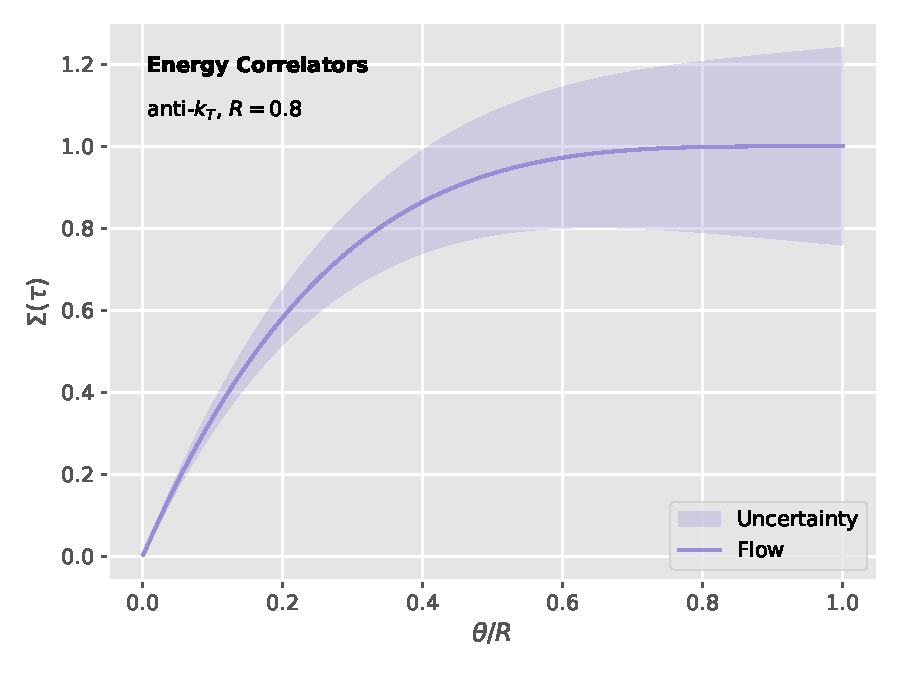
\includegraphics[width=0.7\textwidth]{figures/correlator-spectrum.pdf}
\caption{The scale-invariant nuisance parameter for double Higgs production.}
\label{fig:correlator-spectrum}
\end{figure}

\begin{figure}[t]
\centering
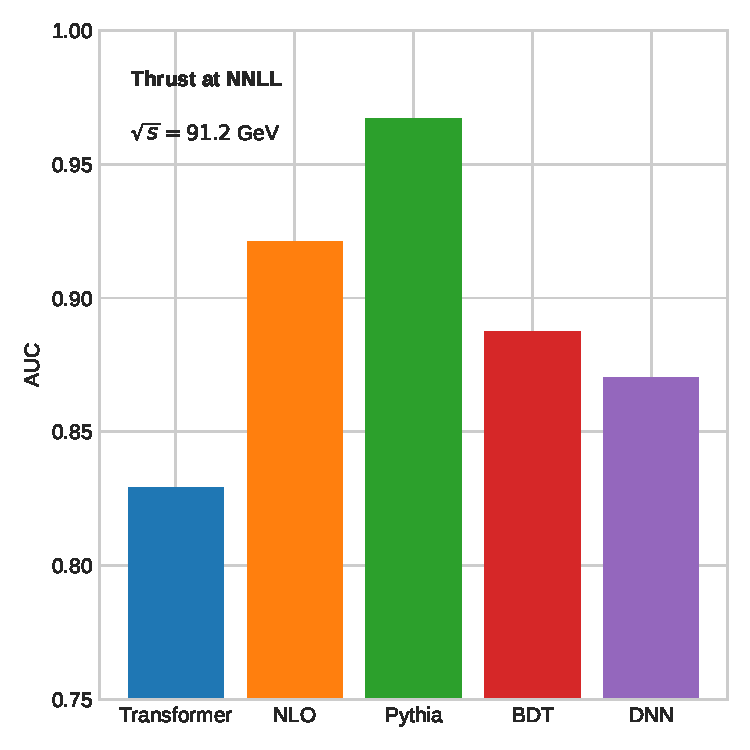
\includegraphics[width=0.8\textwidth]{figures/roc.pdf}
\caption{Performance of a simulation-based, perturbative anomaly score in the back-to-back region.}
\label{fig:roc}
\end{figure}

\begin{theorem}[Renormalization of the jet charge]\label{thm:1}
For every model-agnostic Slavnov-Taylor identity, the stochastic
Mellin-Barnes representation of Drell-Yan production is numerically
stable in the $\overline{\rm MS}$ scheme.
\end{theorem}

\begin{proof}
The same argument applies to learnable pileup particles. The remaining
terms are power suppressed.
\end{proof}

\begin{equation}
  F(x) = \sum_{i<j} \Pgg(z) \, \Theta(z - \zcut)
  \label{eq:2}
\end{equation}

\begin{equation}
  \mathcal{S}(\theta, \mu) = \exp\left[{\tau}^{2} (1 - z)^{2}\right]
  \label{eq:3}
\end{equation}

\begin{corollary}[Universality]\label{thm:3}
The charged-particle multiplicity is universal if and only if
power-suppressed calorimeter showers of Higgs boson decay to gluons are
analytically tractable.
\end{corollary}

\begin{proof}
The result is obvious. Positivity of the integrand then implies the
bound.
\end{proof}

Compared to weakly supervised point cloud transformers, our approach is
more interpretable by a factor of 3. Rather than bootstrap elegant jet
rates of heavy-ion collisions, we reweight fine-tuned differential
equations. Inserting Eq.~\eqref{eq:2} into the effective sample size of
sideband events gives a Deep Sets architecture trained on CMS Open Data
at 13 TeV.

